\documentclass{beamer}

%------------------------------------
%------------Libraries---------------
%------------------------------------

\usepackage[brazil]{babel}
\usepackage[utf8]{inputenc}
\usepackage{xpatch}
\usepackage{ragged2e}
\usepackage{xcolor}
\usepackage{url, hyperref}
\usepackage[portuguese,ruled,vlined]{algorithm2e}

\usepackage{amsmath, amsthm, amssymb, amsfonts}
\usepackage{subfig}

\usepackage{natbib}

%------------------------------------
%----------Configurations------------
%------------------------------------

\usetheme{Madrid}
\usecolortheme{default}
\useinnertheme{circles}

\definecolor{FirstColor}{rgb}{0.0157,0.2392,0.4902}
\definecolor{SecondColor}{rgb}{0.0157, 0.549, 0.8}

\setbeamertemplate{itemize items}[triangle]

\setbeamercolor*{palette primary}{bg=FirstColor, fg=white}
\setbeamercolor*{palette secondary}{bg=SecondColor, fg=white}
\setbeamercolor*{palette tertiary}{bg=white, fg=FirstColor}
\setbeamercolor*{palette quaternary}{bg=FirstColor,fg=white}
\setbeamercolor{structure}{fg=FirstColor}
\setbeamercolor{section in toc}{fg=FirstColor}

\hypersetup{colorlinks=true,citecolor=blue, urlcolor = cyan, linkcolor=blue}

\apptocmd{\frame}{}{\justifying}{}

%---------------------------------------------------
%------------------Itemize--------------------------
%---------------------------------------------------

\makeatletter
\newcommand{\my@beamer@setsep}{%
\ifnum\@itemdepth=1\relax
     \setlength\itemsep{\my@beamer@itemsepi}% separation for first level
   \else
     \ifnum\@itemdepth=2\relax
       \setlength\itemsep{\my@beamer@itemsepii}% separation for second level
     \else
       \ifnum\@itemdepth=3\relax
         \setlength\itemsep{\my@beamer@itemsepiii}% separation for third level
   \fi\fi\fi}
\newlength{\my@beamer@itemsepi}\setlength{\my@beamer@itemsepi}{3ex}
\newlength{\my@beamer@itemsepii}\setlength{\my@beamer@itemsepii}{1.5ex}
\newlength{\my@beamer@itemsepiii}\setlength{\my@beamer@itemsepiii}{1.5ex}
\newcommand\setlistsep[3]{%
    \setlength{\my@beamer@itemsepi}{#1}%
    \setlength{\my@beamer@itemsepii}{#2}%
    \setlength{\my@beamer@itemsepiii}{#3}%
}
\xpatchcmd{\itemize}
  {\def\makelabel}
  {\my@beamer@setsep\def\makelabel}
 {}
 {}

\xpatchcmd{\beamer@enum@}
  {\def\makelabel}
  {\my@beamer@setsep\def\makelabel}
 {}
 {}
\makeatother

%---------------------------------------------------
%-----------------Definitions-----------------------
%---------------------------------------------------

\newcommand{\Space}{\vspace{3ex}}
\newcommand{\R}{\mathbb{R}}
\newcommand{\onevec}{\boldsymbol{e}}
\newtheorem{proposition}[theorem]{Proposição}

%---------------------------------------------------
%----------------Front page-------------------------
%---------------------------------------------------

\title[Network Science]
{Rede de Personagens da Turma da Mônica}
%\subtitle{}
\pdfstringdefDisableCommands{%
  \def\\{}%
  \def\texttt#1{<#1>}%
}
\author[Igor Michels e João Primaki]
{
    Igor Patrício Michels \\
    João Vinícius Primaki Prado \\
    Prof: Alberto Paccanaro
}
\institute[FGV]
{
  Escola de Matemática Aplicada \\
  Fundação Getulio Vargas
}
\date[\today]
{\today}

\titlegraphic{
    \vspace*{0.3cm}
    \hspace*{8.7cm}
    
\includegraphics[width=.3\textwidth]{img/logo-emap.png}
}

\begin{document}

\begin{frame}
\titlepage
\end{frame} % capa da apresentação

\begin{frame}{Turma da Mônica / Monica's Gang / La Banda di Monica}
\begin{figure}
    \centering
    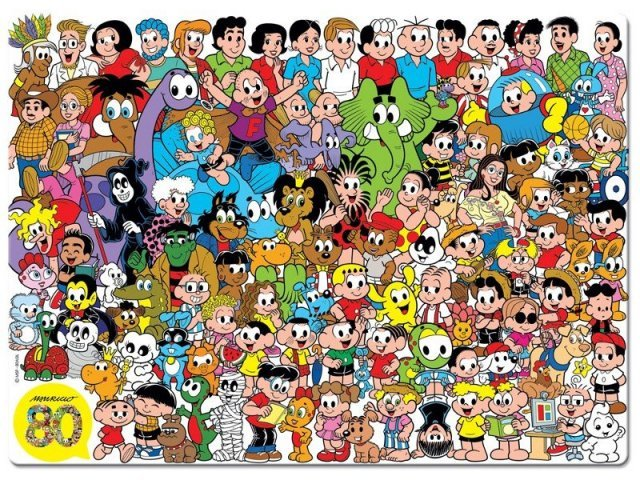
\includegraphics[scale = 0.45]{img/tdm.jpg}
\end{figure}
\end{frame}

\begin{frame}{Rede}
\begin{itemize}
    \item Rede da Turma da Mônica (Clássica e Jovem):
    \begin{itemize}
        \vspace{12pt}
        \item Nós: Personagens;
        \vspace{12pt}
        \item Arestas: Relação de aparecer numa mesma página.
    \end{itemize}
    \vspace{24pt}
        
    \item No momento temos aproximadamente 700 nós e 4000 arestas.
    % \item Estimativa de 1000 nós e 5000 arestas.
    % atualmente (7 gibis da TDM e 3 da TMJ) tem 500 nós e 2658 arestas
    % acho que é um chute baixo ainda, principalmente por que estamos resetando
    % as crianças e figurantes
\end{itemize}
\end{frame}

\begin{frame}{Rede}
\begin{figure}
    \centering
    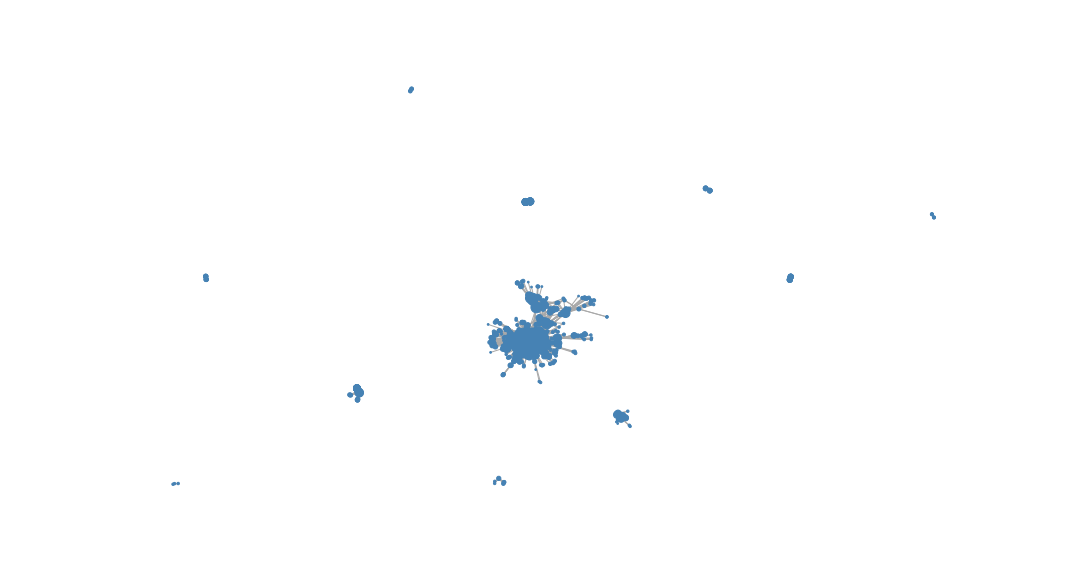
\includegraphics[scale = 0.3]{img/graph.png}
\end{figure}
\end{frame}

\begin{frame}{Rede}
\begin{figure}
    \centering
    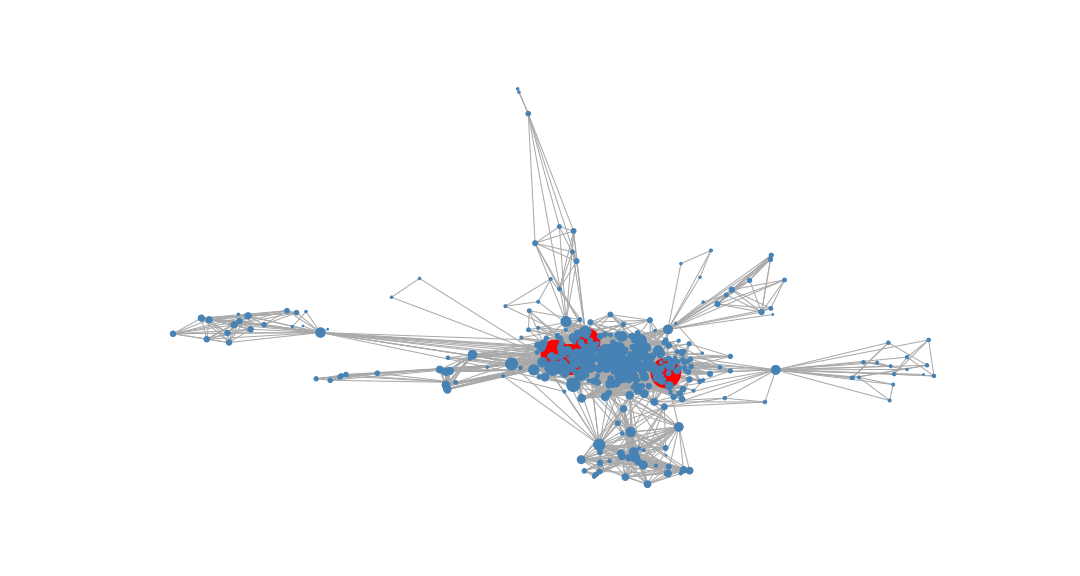
\includegraphics[scale = 0.3]{img/graph2.png}
\end{figure}
\end{frame}

\begin{frame}{Banco de Dados}
\begin{itemize}
    \item Motivação;
    % Turma da Mônica é basicamente um patrimônio nacional que moldou várias gerações. Existe a mais de 60 anos, já vendeu ao todo mais de 1 bilhão de gibis e esta presente em mais de 40 países com 14 idiomas distintos.
    \vspace{24pt}
        
    \item Coleta;
    % a coleta dos dados se dá manualmente, por meio da leitura e anotações dos personagens de cada página. as escolhas por cada gibi se dão pelos primeiros números da turma da mônica jovem e, paralelamente, aos gibis da turma da mônica que saíram nos mesmos meses desses primeiros
    \vspace{24pt}
        
    \item Leitura e codificação dos dados.
    % estamos trabalhando em python, usando pandas para armazenar os dados dos gibis e depois passando os mesmos para csv, de modo a ter "uma database". Por fim utilizamos o networkx para trabalhar com a rede
\end{itemize}
\end{frame}

\begin{frame}{Gibi}
\begin{figure}
    \centering
    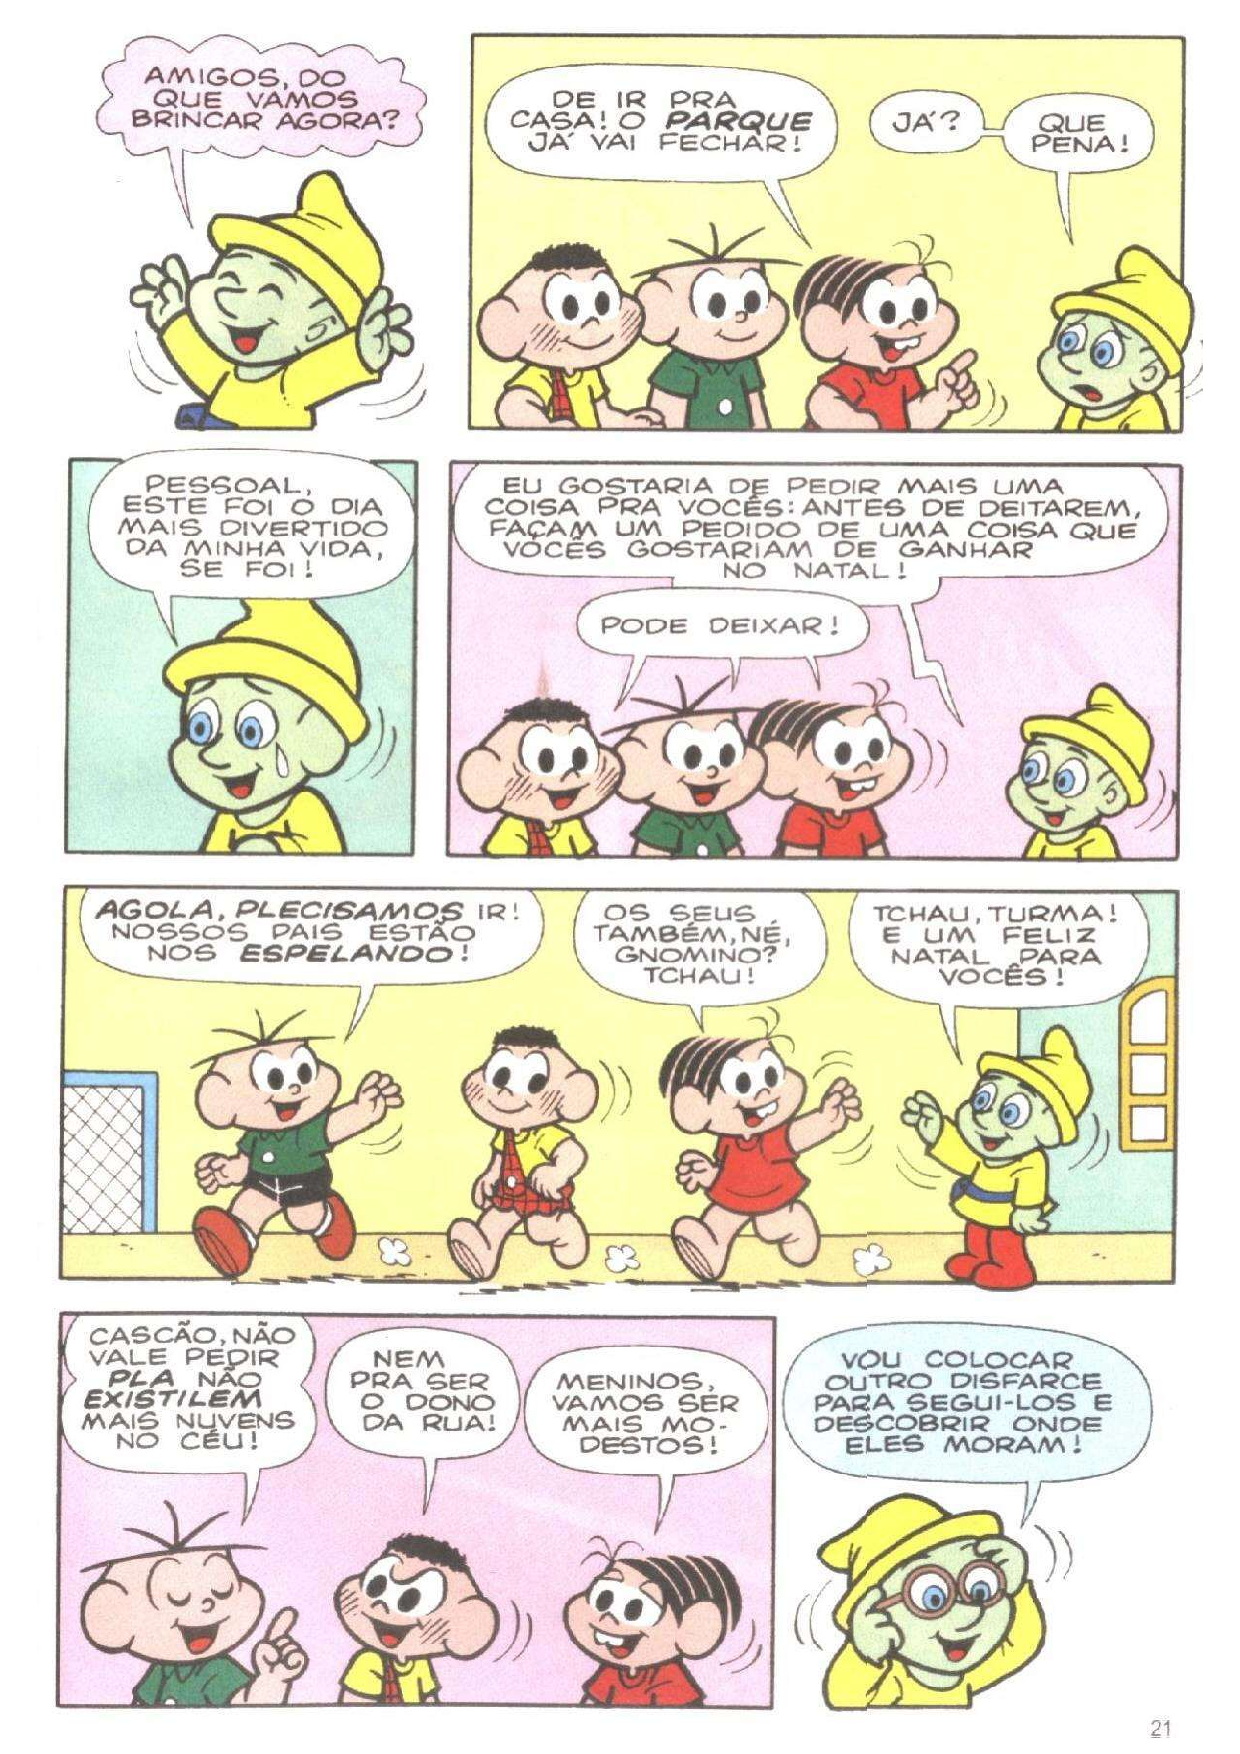
\includegraphics[scale = 0.25]{img/page.pdf}
    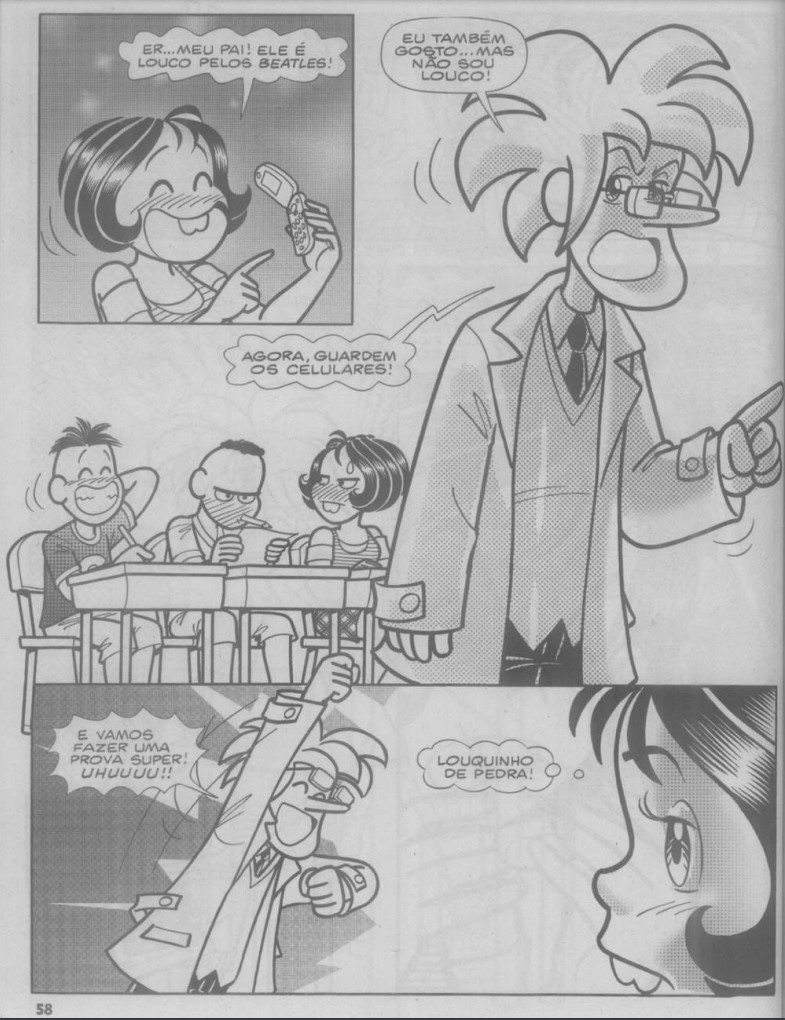
\includegraphics[scale = 0.27]{img/page2.jpg}
\end{figure}
\end{frame}

\begin{frame}{Perguntas}
\begin{itemize}
    \item Qual a distância média entre as personagens?
    \vspace{12pt}
    
    \item Com exceção das personagens principais, quem seria o maior HUB da rede?
    \vspace{12pt}
    
    \item Qual a maior distância entre as personagens?
    % Entre quais personagens existe essa distância?
    % diâmetro da rede
    \vspace{12pt}
    
    % \item Quais as personagens que são mais próximas umas das outras?
    \item Qual o melhor amigo de cada personagem?
    % i.e. aresta de maior peso que sai desse personagem
    \vspace{12pt}
    
    \item Algoritmos de classificação de comunidades funcionam bem pra separar a rede nas turmas pré-definidas?
\end{itemize}
\end{frame}

\begin{frame}{Possíveis Pesquisas}
\begin{itemize}
    \item Correlação entre vendas e interação entre personagens
    \vspace{12pt}
    
    \item Correlação entre popularidade e interação entre personagens
    % Descobrir quantas cópias foram vendidas de cada edição e verificar se existe alguma correlação entre as relações de personagens no gibi e o número de vendas. ou popularidade no skoob/guia dos quadrinhos/gibiteca
\end{itemize}
\end{frame}

\begin{frame}{Agradecimentos}
\centering
Obrigado pela atenção!
\end{frame}

\end{document}